\chapter{Event reconstruction}
Interpreting the detector signals and reconstructing the event along with the associated objects relies on a number of sophisticated algorithms. The current chapter provides superficial overview of these algorithms that allow to reconstruct particles (electrons, photons, muons etc) and event-related parameters like the coordinates of the primary vertex.
    \section{Charged particles track reconstruction}
    \label{sec::tracking}
    A track $q$ is formed based on the information from the \gls{id} and is represented by five parameters: $q = (d_0,z_0,\phi,\theta,q/p)$, where $d_0$ is the distance from the track to the Z axis (transverse impact parameter), $z_0$ is the Z coordinate of the perpendicular dropped from the track onto the Z axis (longitudinal impact parameter) (see fig. \ref{fig::z0d0}), $\phi$ and $\theta$ are the azimuthal and polar angles correspondingly and $q/p$ is the charge to momentum ratio of the particle. The process for track reconstruction is the same for lepton and charged hadron candidates. 
    
        	\begin{figure}[htbp]
        		\centering
    		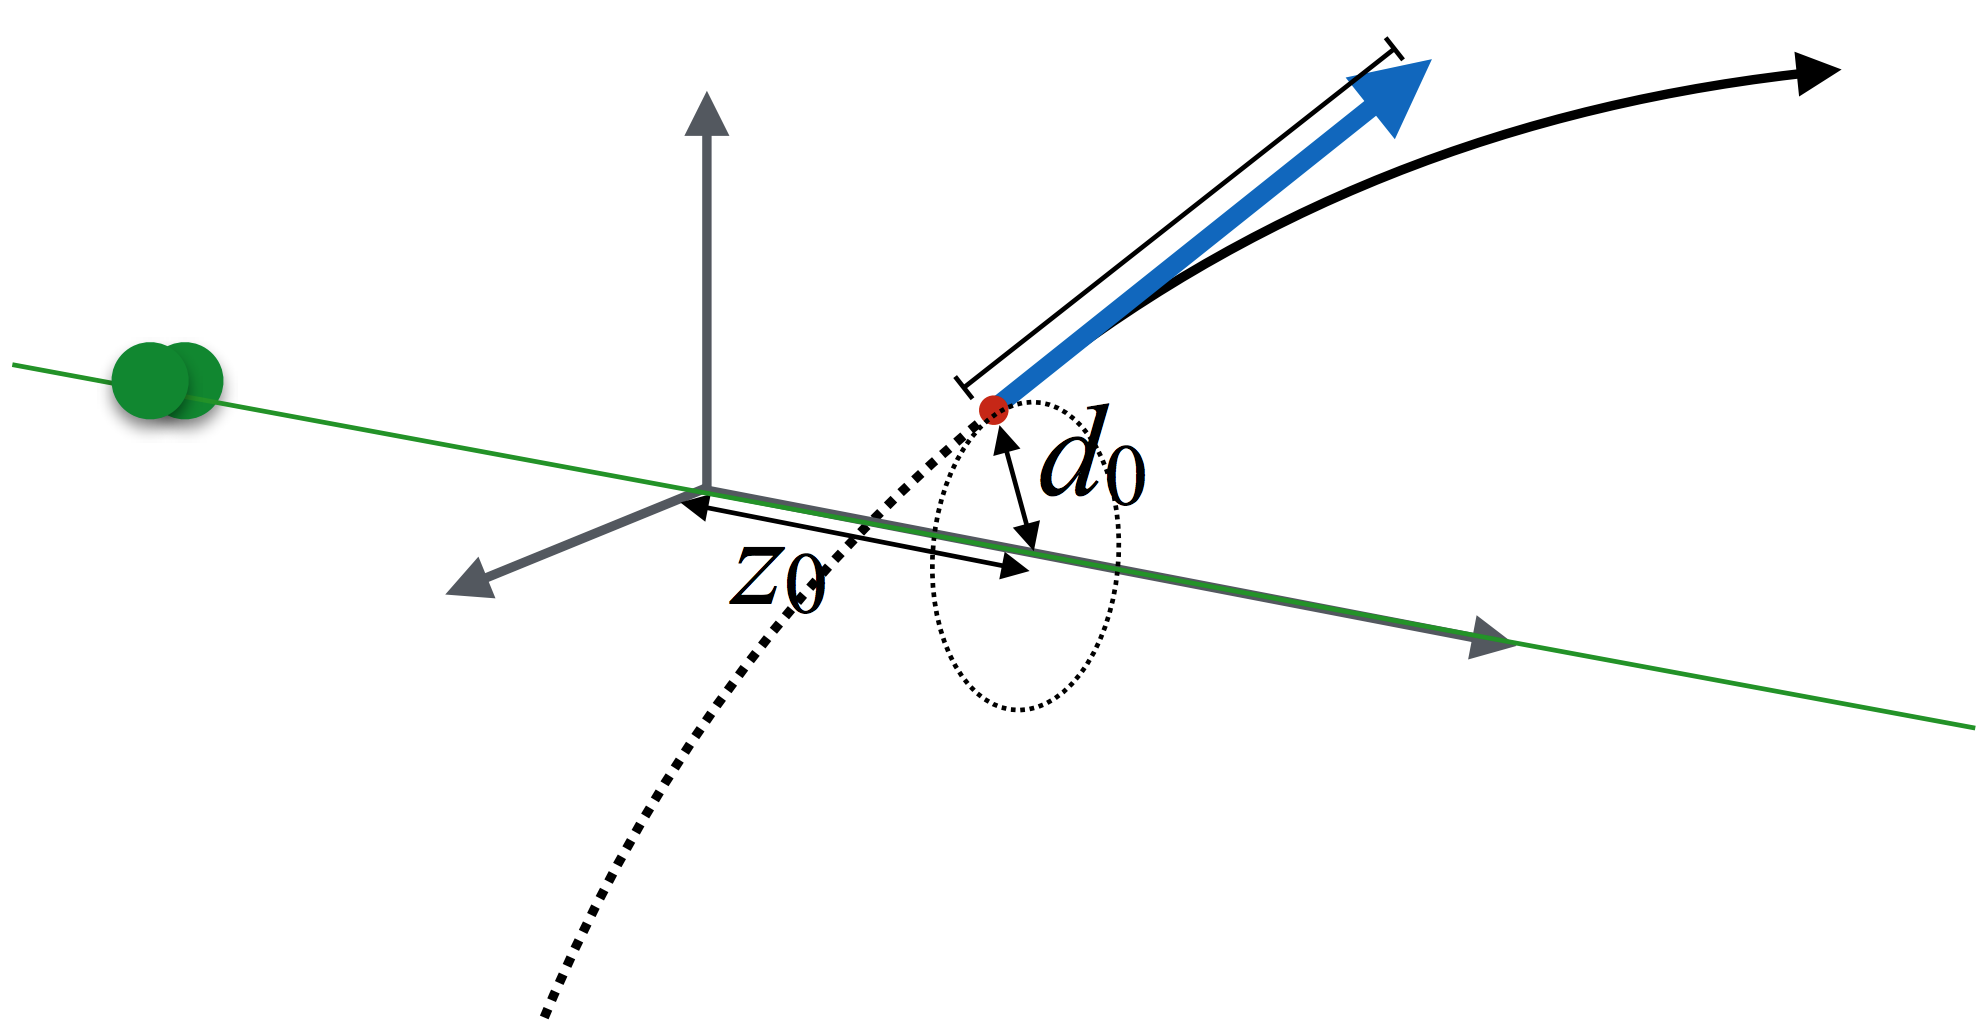
\includegraphics[width=0.5\textwidth,keepaspectratio]{track_coord.png}
    		\caption[Impact parameters]{Impact parameters $z_0$ and $d_0$ \cite{ATLAS:track}.}
    		\label{fig::z0d0}
  			 \end{figure}
  	To form tracks using the detector response information the following steps are performed \cite{ATLAS:track2}:
  	\begin{itemize}
  		\item \textbf{Clustering} single hits in the pixel and SCT detectors. Neighbouring hits are combined to form a single cluster, clusters are then transformed into \textit{space points} that have having 3D coordinates. A cluster may be identified as a single-particle cluster or as merged cluster, created by two or more particles. Identification of a cluster as a merged one and separation of energy deposits between the particles (possible only for two particles) is performed by means of a \gls{nn} algorithm. 
  		\item \textbf{Forming seeds} out of the space points. To form a seed three space-points originating from unique layers of the silicon detectors (pixel or SCT) are used. All possible combinations of seeds are formed at this stage. For every seed a crude estimate of the track parameters is performed. 
  		\item \textbf{Track candidates} are formed out of the seeds by extending them within the silicon sub-detectors following the most likely path. A combinatorial Kalman filter \cite{Fruhwirth:1987fm} is used to build the track candidates. The purity of the seeds depends significantly on the sub-detector that recorded the corresponding space-points. SCT-only seeds are considered the most reliable, followed by the seeds that origin only from the pixel detector space-points, and the least reliable are the seeds originating from both of these sub-detectors -  that determines the order of seed consideration when composing track candidates. \\Some fraction of the seeds that meet the necessary requirements become track candidates, the rest are discarded. A seed may be used for more than one track candidate if more than one space-point extension exists on the same layer.
  		\item \textbf{Ambiguity solving} is the next step necessary to eliminate incorrectly assigned space-points or resolve conflicting track candidates that have an overlapping space-point. At this stage the track candidates are assigned a \textit{track score}. The track score depends on the number of clusters associated to the track and which sub-detector these clusters originate from, the existence of holes (the absence of a cluster associated to a detector layer crossed by the track), the quality of the $\chi^2$ fit of the track and track momentum.
  		
  		The tracks are ordered by their track score and consequently fed to the ambiguity resolving sequence. A track must pass a number of kinematic cuts, impact parameters cuts, number of holes, number of clusters and shared clusters cuts, otherwise the track candidate is rejected. If a track candidate has no shared clusters with other candidates it is accepted after that. If there are merged clusters then it is up to the \gls{nn} to either accept the track, reject it or eliminate a space-point and recycle the updated track candidate (see Fig. \ref{fig::tr_ambig}). 
  		\item \textbf{TRT extension} means matching of the track, composed using the information from silicon sub-detectors to the trace in the TRT tracker. This allows to improve momentum measurement benefiting from extended track length.
  		\item Final high-resolution \textbf{track fit} is performed using all available information. Position and uncertainty of each cluster are determined by an additional \gls{nn} allowing for more precise track parameters. The curvature of the particle track also serves for charge sign identification.
  	\end{itemize}
  		\begin{figure}[htbp]
  		\begin{subfigure}[t]{0.65\textwidth}
  			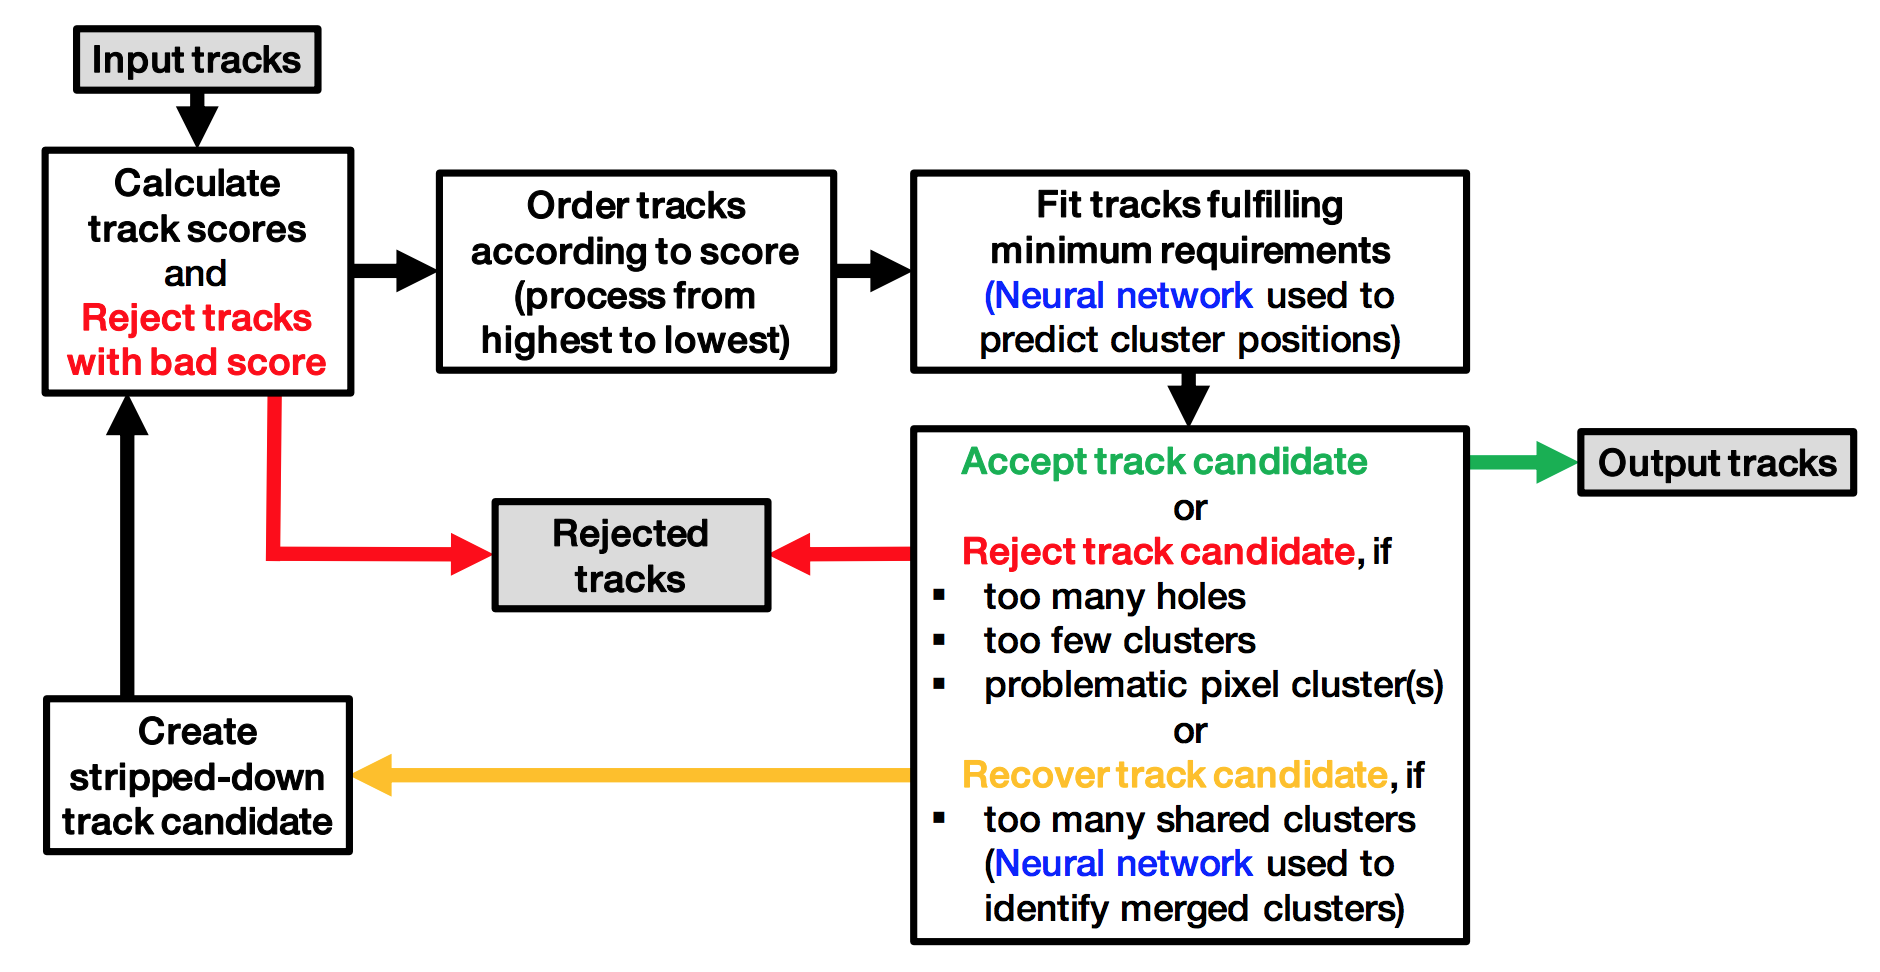
\includegraphics[width=\textwidth,keepaspectratio]{track_ubmig.png}
  			\caption[Side view]{Track ambiguity resolver algorithm.}
  			\label{fig::tr_ambig}
  		\end{subfigure}
  		\hfill
  		\begin{subfigure}[t]{0.33\textwidth} 
  			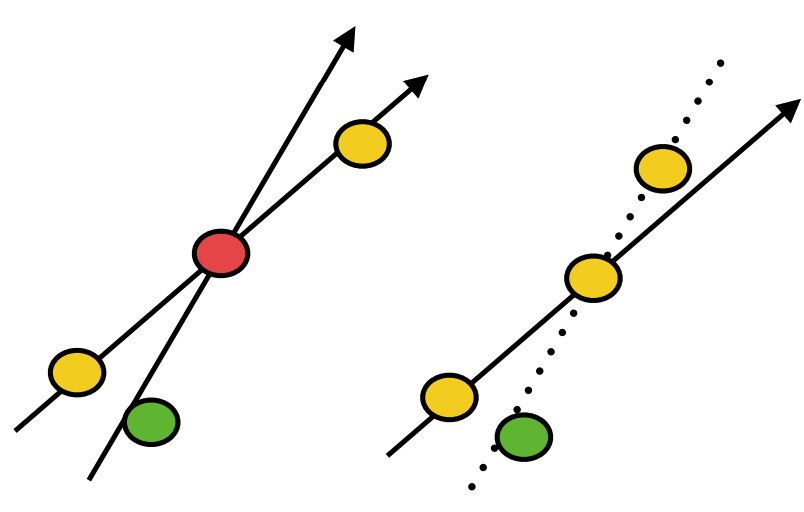
\includegraphics[width=\textwidth,keepaspectratio]{track_overlap.png}
  			\caption[Tracks sharing space-points]{Tracks sharing space-points.}
  			\label{fig::tr_overlap}
  		\end{subfigure}
  		\caption{Ambiguity solving process~\cite{ATLAS:track2}.}
  		\label{fig::tr_resol}
  	\end{figure}
  \section{Determining the primary vertex of the event}
   Primary vertex determination is crucial for physics analyses for many  reasons. One of them is the necessity to separate particles originating from hard events from pile-up. Another reason is to keep track of long-lived decay chains and distinguish between prompt and non-prompt particles. Flavour tagging, background suppression and decay reconstruction also rely heavily on the primary vertex determination.
   
  After reconstructing the tracks of individual particles the obtained information is used to reconstruct the \gls{pv} of the event \cite{PrimVertRun12}. The procedure relies on the reconstructed tracks and goes as follows:
  \begin{itemize}
  \item A seed from the first vertex is selected. The transverse position of the seed is taken as the centre of the beam spot. The z-coordinate of the seed is calculated as the mode of $z_0$ coordinates of the tracks.
  \item Using the seed and the available tracks an iterative fit is performed in order to find the best position for the \gls{pv}. In each iteration the tracks that are less compatible with the vertex are down-weighted and the vertex position gets recomputed. With every iteration the spread in the weight increases, separating track set into compatible tracks that mostly determine the vertex position and incompatible tracks that have little weight and therefore very little influence on the track position. 
  \item After the fit is done compatible tracks remain assigned to the vertex, while incompatible tracks are removed from it. These incompatible tracks can be used in the determination of a different vertex.
  \item The procedure is repeated with the remaining tracks of the event. 
  \item The primary vertex is a vertex with the highest sum of the assigned tracks transverse momenta $\sum_{tracks}p_T^{2}$.
  \end{itemize}  
  For the upcoming Run 3 of the LHC certain improvements and modifications are foreseen \cite{PrimVertRun3}.
  \begin{figure}[htbp]
  	\centering
  	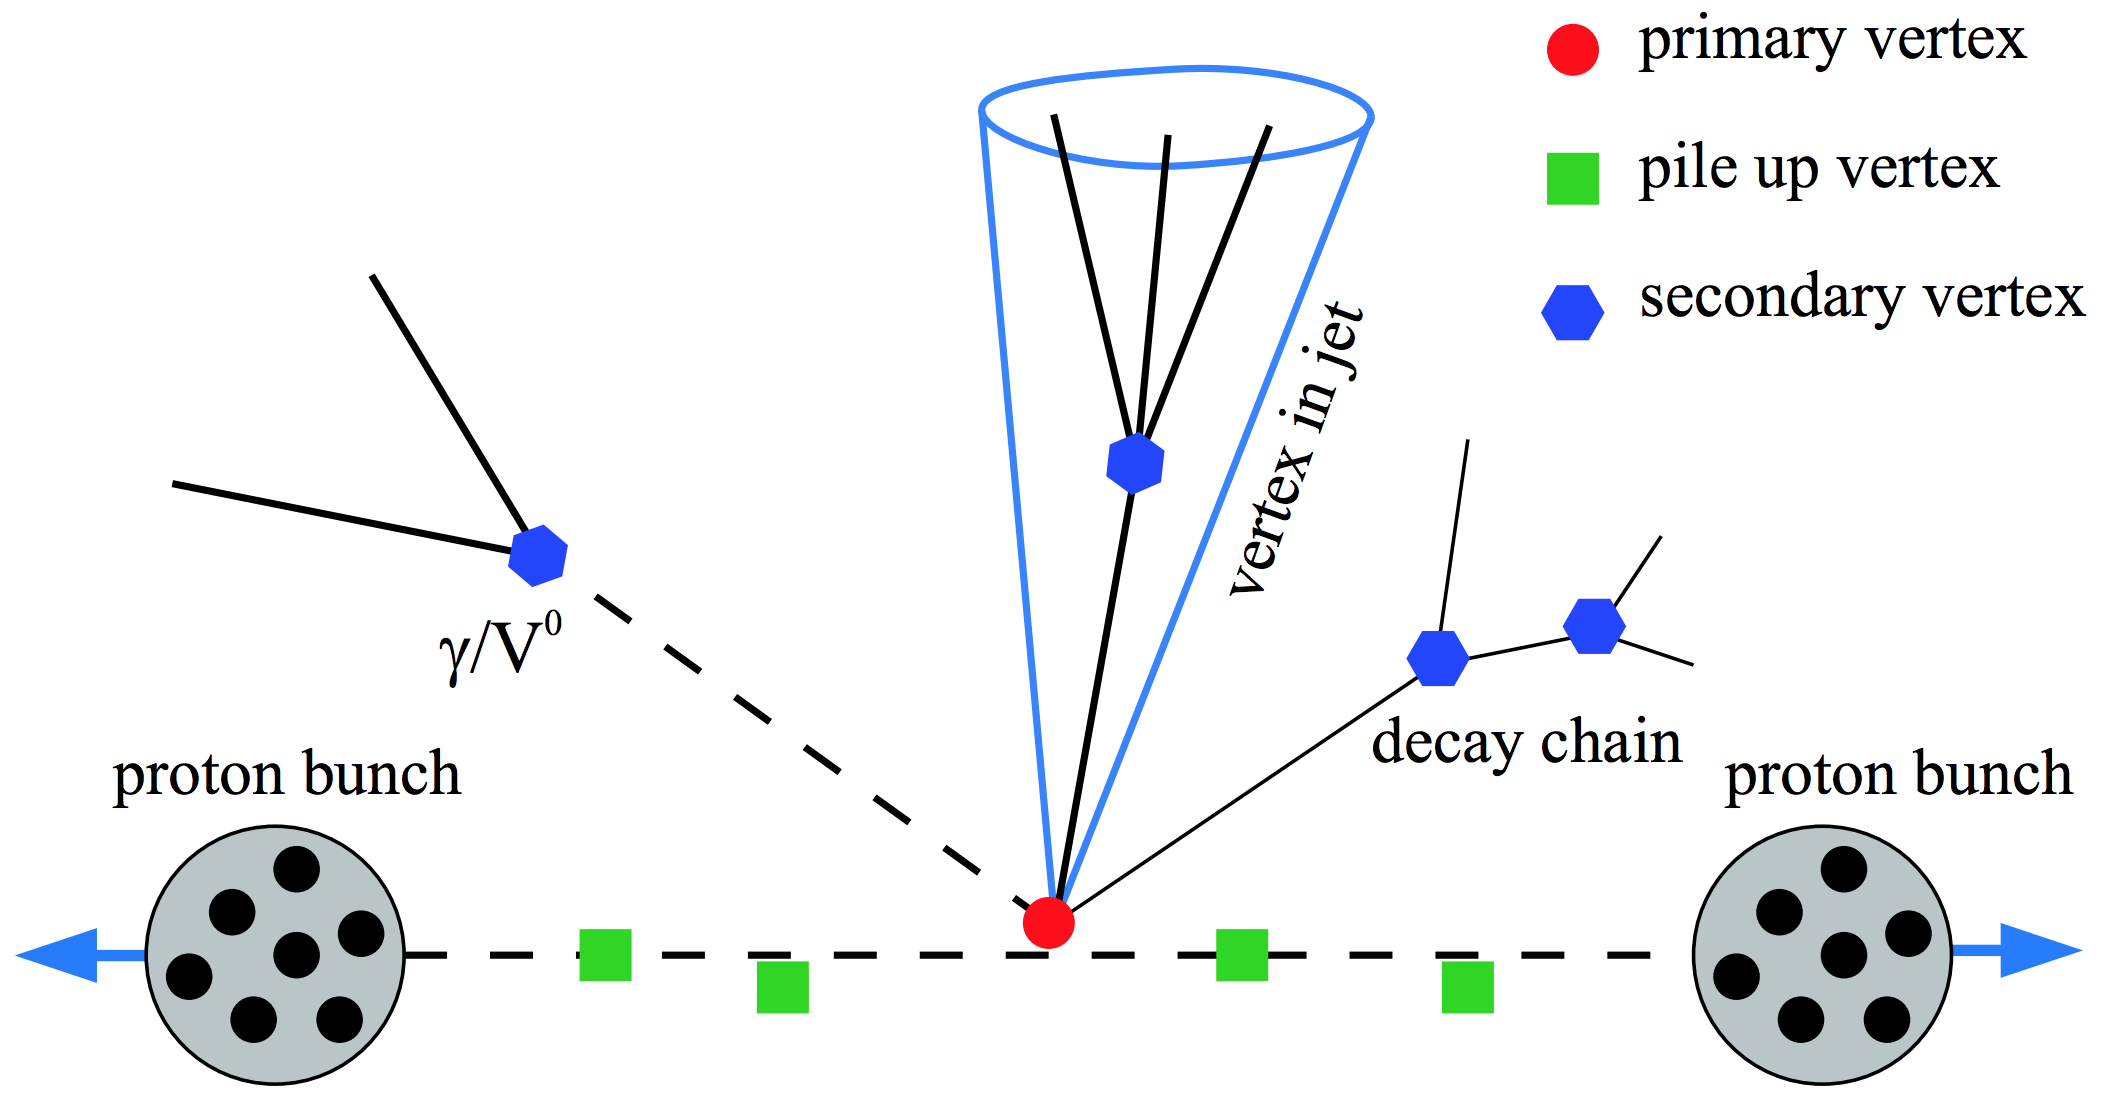
\includegraphics[width=0.5\textwidth,keepaspectratio]{primary_vertex.png}
  	\caption[Types of vertices]{Primary, secondary and pile-up vertices \cite{vert_recon}.}
  	\label{fig::pv}
  \end{figure}
    \section{Muon reconstruction and identification}
    Muon reconstruction relies primarily on the information from the \gls{id} (the muon track) and the \gls{ms}, sometimes also using additional information from the calorimeter. At the first stage a muon is independently reconstructed in the tracker and in the spectrometer, and then the two reconstructed tracks are combined to compose a muon track used in the physics analyses \cite{muons_reco1}. Track reconstruction is described in section \ref{sec::tracking}. 
    \subsection{Muon reconstruction}
    Muon reconstruction in the muon spectrometer begins with a search for hit patterns in each muon chamber and forming of the segments. Using the Hough transform \cite{ILLINGWORTH198887} the hits in each MDT chamber and nearby trigger chamber are aligned on trajectories in the bending plane. The orthogonal coordinate is measured with RPC and TGC detectors. A separate combinatorial search is conducted in the CSC detectors in $\phi$ and $\eta$ detector planes.\\
     \begin{figure}[htbp]
    	\centering
    	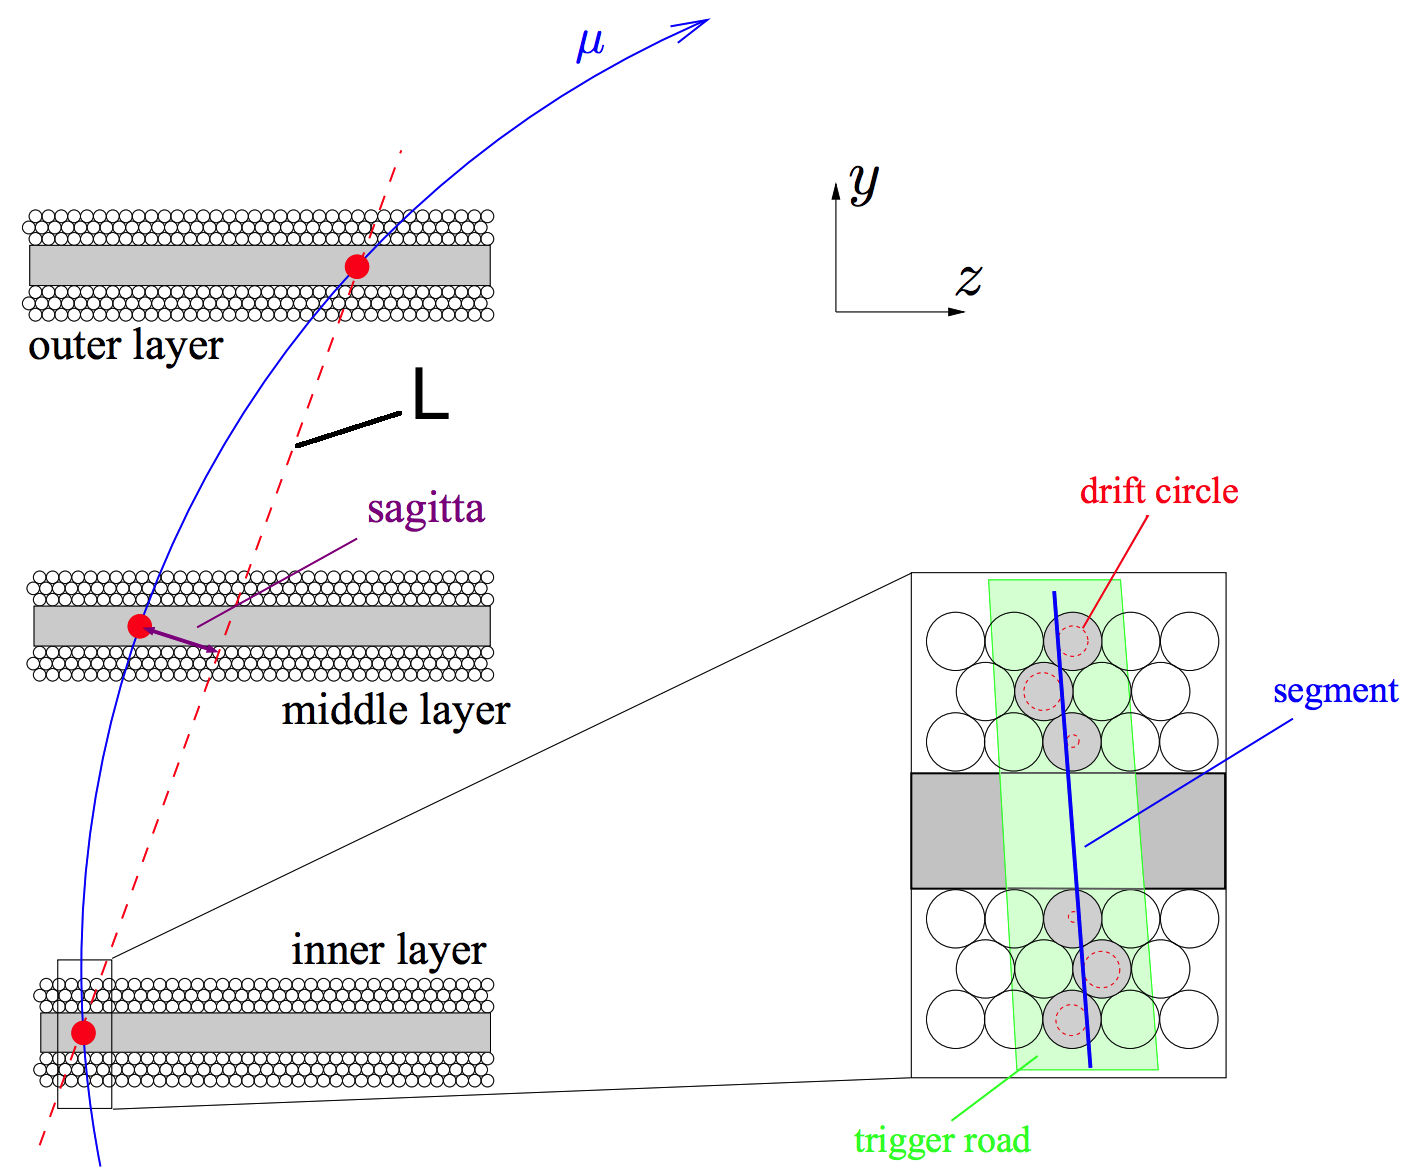
\includegraphics[width=0.5\textwidth,keepaspectratio]{sagitta.png}
    	\caption[Muons sagitta]{Sagitta used for the determination of the muon momentum \cite{Kaiser:2010zea}.}
    	\label{fig::sagitta}
    \end{figure}
    Then the track candidates are built by fitting hits from different layers. This algorithm starts a combinatorial search first using the segments from the middle layers as seeds, as there are more trigger hits in the middle layer. The search is later extended to include the segments from other layers as seeds. Segment selection criteria are based on hit multiplicity and fit quality. The segments are matched using their relative positions and angles. In all the regions, except barrel-endcap transition region, at least two matching segments are needed to build a track (one segment is enough in the transition region).
    
    A single segment can be used by two or more track candidates. An overlap removal algorithm decides to which track should a segment belong or shares a segment between two tracks. A global $\chi^2$ fit is used to fit all the hits associated to every track. If the $\chi^2$ fit meets the designated criteria then the track is accepted. If a hit impair the $\chi^2$ fit significantly, then this hit may be removed and the fit is repeated. On the other hand, new hits may be recovered if they fit the track candidate trajectory. 
    
    Accurate fitting of the track trajectory is extremely important for the measurement of muon momentum. A quantity called \textit{sagitta} is measured by the \gls{ms} (see Fig. \ref{fig::sagitta}). Knowing the length $L$ and the sagitta $S$ we can determine the momentum:
    	\begin{equation}
    p = \frac{BL^2}{8S},\\
    \end{equation}
    where $B$ is the magnetic field strength.
    
    After the muon gets reconstructed in every detector system separately, the obtained information is combined to form a reconstructed muon object. Depending on the detectors used for the combined reconstruction there are \textit{four types of muons} defined (see Fig. \ref{fig::muon_combined}):
    \begin{itemize}
	\item \textbf{Combined (CB) muon} is formed from a global refit of the tracks reconstructed independently in the \gls{id} and in the \gls{ms}. During this global refit the hits from both detectors are used and also new hits may be added. Normally the outside-in pattern is used, when \gls{ms} track is extrapolated inwards to match \gls{id} track. Inverse inside-out procedure is used as a complementary approach.
	\item \textbf{Segment-tagged (ST) muon} is a particle with an \gls{id} track that was extrapolated to the \gls{ms} and associated with at least one local track segment in the MDT or CSC chambers. Normally these are muons with low $p_T$ or their trajectory crosses regions with reduced \gls{ms} acceptance.
	\item \textbf{Calorimeter-tagged (CT) muon} has a valid \gls{id} track that can be associated to an energy deposit in the calorimeter compatible with minimum-ionizing particle. The CT muons have the lowest purity among the muon types although they provide acceptance where the \gls{ms} coverage may be absent, like the very central region with $|\eta| \le 0.1$ for $15<p_T<100$ GeV. 
	\item \textbf{Extrapolated (ME) muon} (standalone muon) trajectory is reconstructed base only on the \gls{ms} track and a loose requirement to match the \gls{ip}. ME muons allow to extend the muon acceptance to the region which is not covered by the \gls{id}, namely $2.5<|\eta| < 2.7$.
	\end{itemize}
	In case of overlap between different muon types the preference is given to CB muons, then to ST and then to CT muons. ME muons overlaps are resolved based on the \gls{ms} track quality.
      \begin{figure}[htbp]
	\centering
	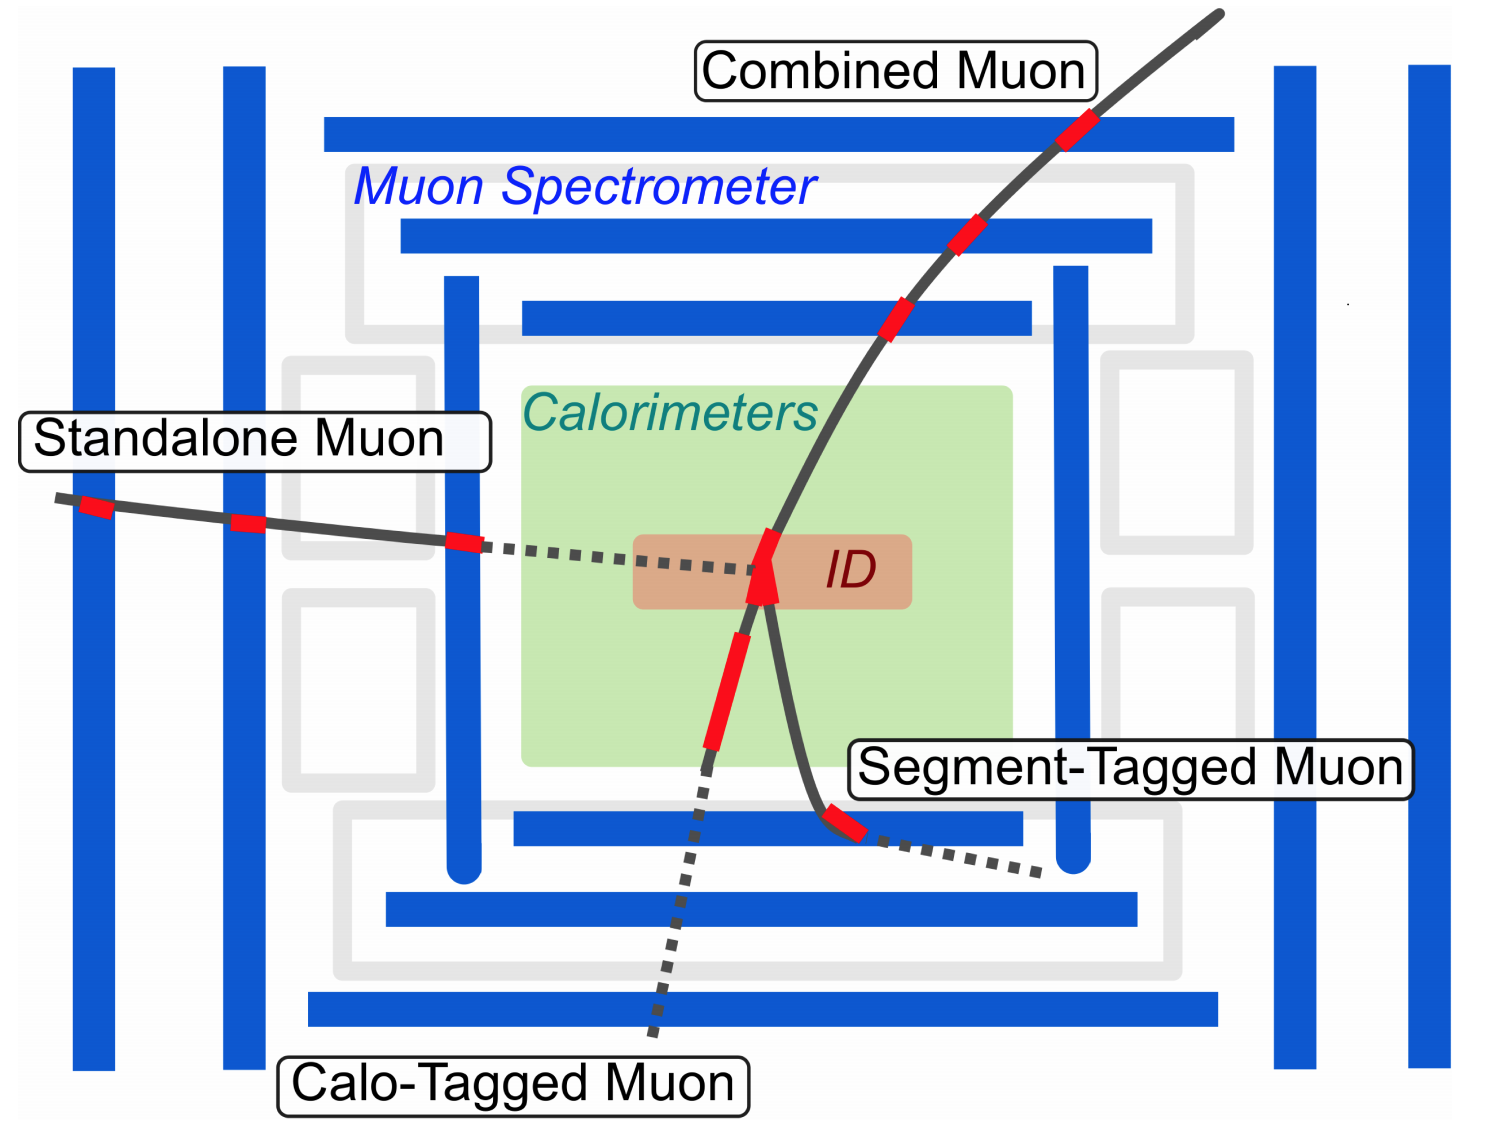
\includegraphics[width=0.5\textwidth,keepaspectratio]{muons_info.png}
	\caption[Reconstructed muon types]{The four types of reconstructed muons~\cite{muons_reco1}.}
	\label{fig::muon_combined}
	\end{figure}
     \subsection{Muon identification}
     Muon identification is a set of measures to ensure that the registered particle has indeed the characteristics of a muon and to identify the mechanism of its production. Muons created in the course of decay of a short-lived particle (e.g. a massive boson) are called \textit{prompt muons}, while those originating from hadron or tau decays are called \textit{non-prompt}. Muon identification plays an important role in background suppression and guaranteeing a robust momentum measurement.
     
     Muons that are created during the in-flight decay of the charged hadrons in the \gls{id} usually have a distinctive "kink" topology in their reconstructed track. This results in a decreased quality of the resulting track fit and the incompatibility between the results of momentum measurement in the \gls{id} and \gls{ms}. Muons originating from W boson decays are called \textit{signal}, while those coming from hadron decays are called \textit{background}. For CB muons the three main identification variables are the following:
     \begin{itemize}
    	\item \textit{q/p significance} is defined as $\frac{|(q/p)_{ID}-(q/p)_{MS}|}{\sqrt{\sigma^2(q/p)_{ID}+\sigma^2(q/p)_{MS}}}$ - an absolute difference between $q/p$ measured in the two detectors over the combined uncertainty.
    	\item Relative transverse momentum difference $\rho = \frac{|p_T^{ID}-p_T^{MS}|}{p_T^{combined}}$.
    	\item Normalized $\chi^2$ fit of the combined track.
 	\end{itemize}
 	Robust momentum measurement is ensured by specific requirements to the number of hits in the \gls{id} and \gls{ms}. A number of muon identification selections (working points) is developed to address specific analyses. 
     \subsection{Muon isolation}   
     Isolated muons are a defining signature of massive boson decays. In the decays of W, Z and Higgs bosons muons are created separated from the rest of the particles. Quantitative measurement of detector activity around a muon candidate is called \textit{muon isolation} and serves as an invaluable tool for background suppression. Muon isolation is assessed through two observables: one is track-based, another is calorimeter-based. 
     
     The track-based observable $p_T^{varcone20}$ is defined as a scalar sum of all the particles with $p_T>1$ GeV in a cone $\Delta R=min(10 GeV/p_T^{\mu},0.2)$ around the muon with transverse momentum $p_T^{\mu}$ excluding the proper track of the muon. The $p_T$ dependence helps this definition to perform better for the muons created in the decay of the particles with high transverse momentum.
     
     The calorimeter-based isolation observable $E_T^{topocone20}$ is defined as the sum of the transverse energy of all the topological clusters in a cone of a size $\Delta R = 0.2$ around the muon after subtracting the proper muon energy deposit and correcting for the pile-up effects.
     
     In both cases the size of the cone may be varied, normally in the range between 0.2 and 0.4, depending on the analysis needs. Isolation criteria are typically defined using the relative isolation variables, using the ratio of  $p_T^{varcone20}$ and $E_T^{topocone20}$ to the transverse momentum. A number of working points exist, each having a certain requirements for one or both of the isolation variables.
     
     \section{Electron reconstruction and identification}
     \subsection{Electron reconstruction}
           \begin{figure}[htbp]
     	\centering
     	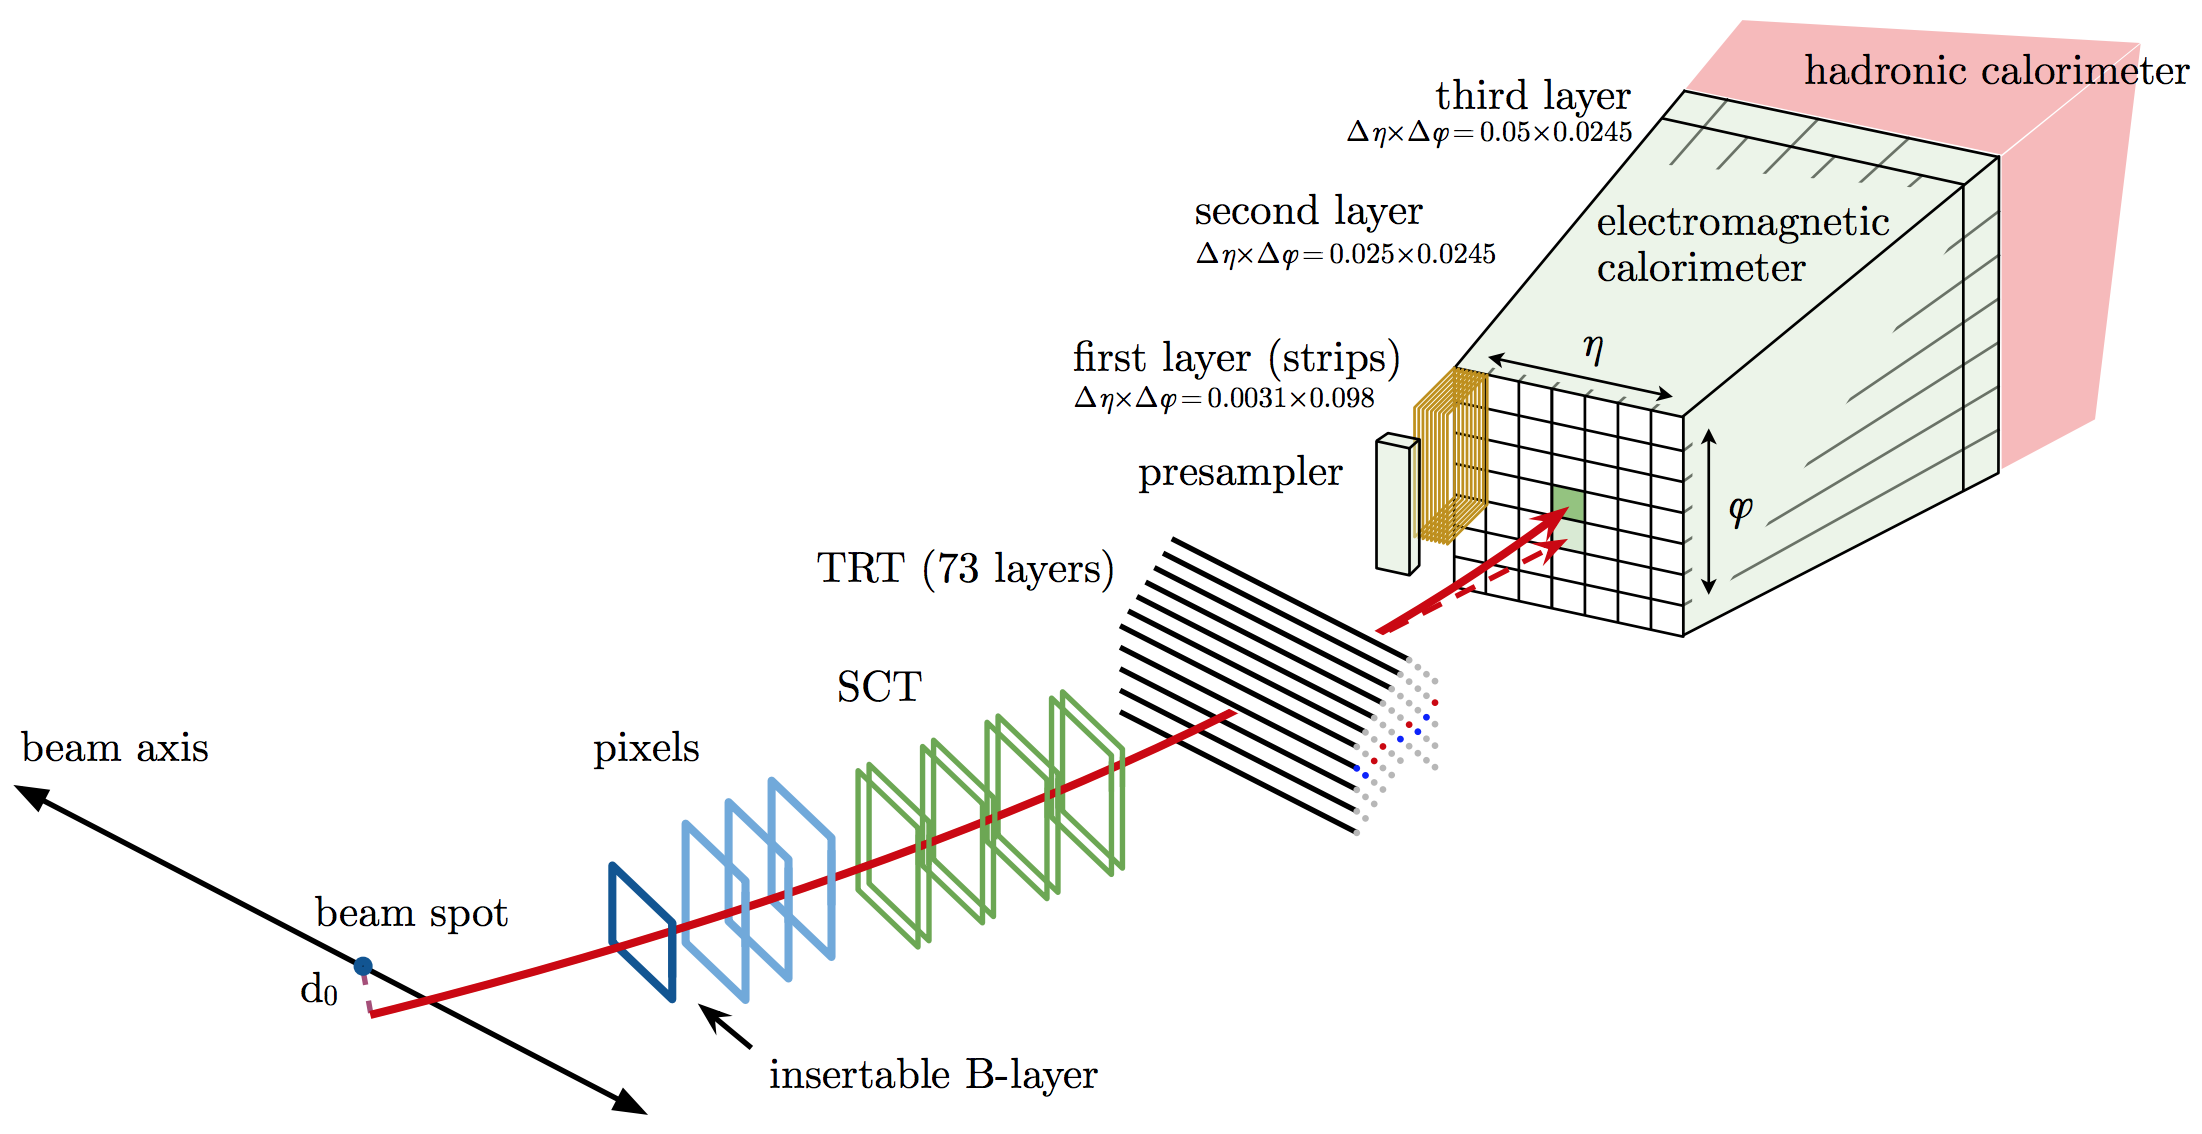
\includegraphics[width=\textwidth,keepaspectratio]{el_scheme.png}
     	\caption[Electron path]{The path of an electron through the detector is shown by solid red line. The dashed red line denotes the trajectory of a photon, produced as a Bremsstrahlung radiation in the TRT~\cite{electrons_reco1}.}
     	\label{fig::el_id_scheme}
     \end{figure}
     Electron reconstruction starts with two separate parts: track reconstruction in the \gls{id} and cluster reconstruction in the calorimeter, which are then matched to each other in order to make an electron candidate \cite{electrons_reco1}. During Run 2 two algorithms were used for the cluster reconstruction, both of them are described below.
     
     \subsubsection{Sliding window}
     It must be mentioned that this method is deprecated and starting from 2017 is replaced by the topocluster method described in the next section. 
     The \gls{emc} is divided into a grid of 200x256 towers in $\eta \times \phi$ plane, each tower having a size of $\Delta \eta \times \Delta \phi=0.025\times0.025$, reproducing the granularity of the second layer in the \gls{emc}. Energy deposits in all available calorimeter layers (first, second and third layers of the \gls{emc} in the region $|\eta| < 2.47$ and the presampler in the region $|\eta| < 1.8$) are approximately calibrated at the EM scale and summed up for each tower. If the cumulative energy deposit in a certain tower exceeds 2.5 GeV then this tower is used as a seed. Then for every seed a sliding window algorithm of size $3 \times 5$ is used \cite{Lampl:1099735}, forming a cluster around every seed. 
     
     It happens that two seed-cluster candidates are found in close proximity. When their towers overlap within an area of $\eta \times \phi=5\times 9$ in units of $0.025\times0.025$ the two clusters are considered overlapping. In this case two options are possible:
      \begin{itemize}
     	\item If the transverse energies of the two clusters are more than 10\% different then the cluster with higher $E_T$ is retained.
     	\item If the difference in the transverse energies is within 10\% then the cluster with higher value of the $E_T$ in the central tower is kept.
     \end{itemize}
 	After the overlap is resolved the duplicate cluster is removed.\\
 	 \subsubsection{Topocluster reconstruction}
 	  	 	\label{sec::topocluster}
 	  	\begin{figure}[htbp]
 	 	\centering
 	 	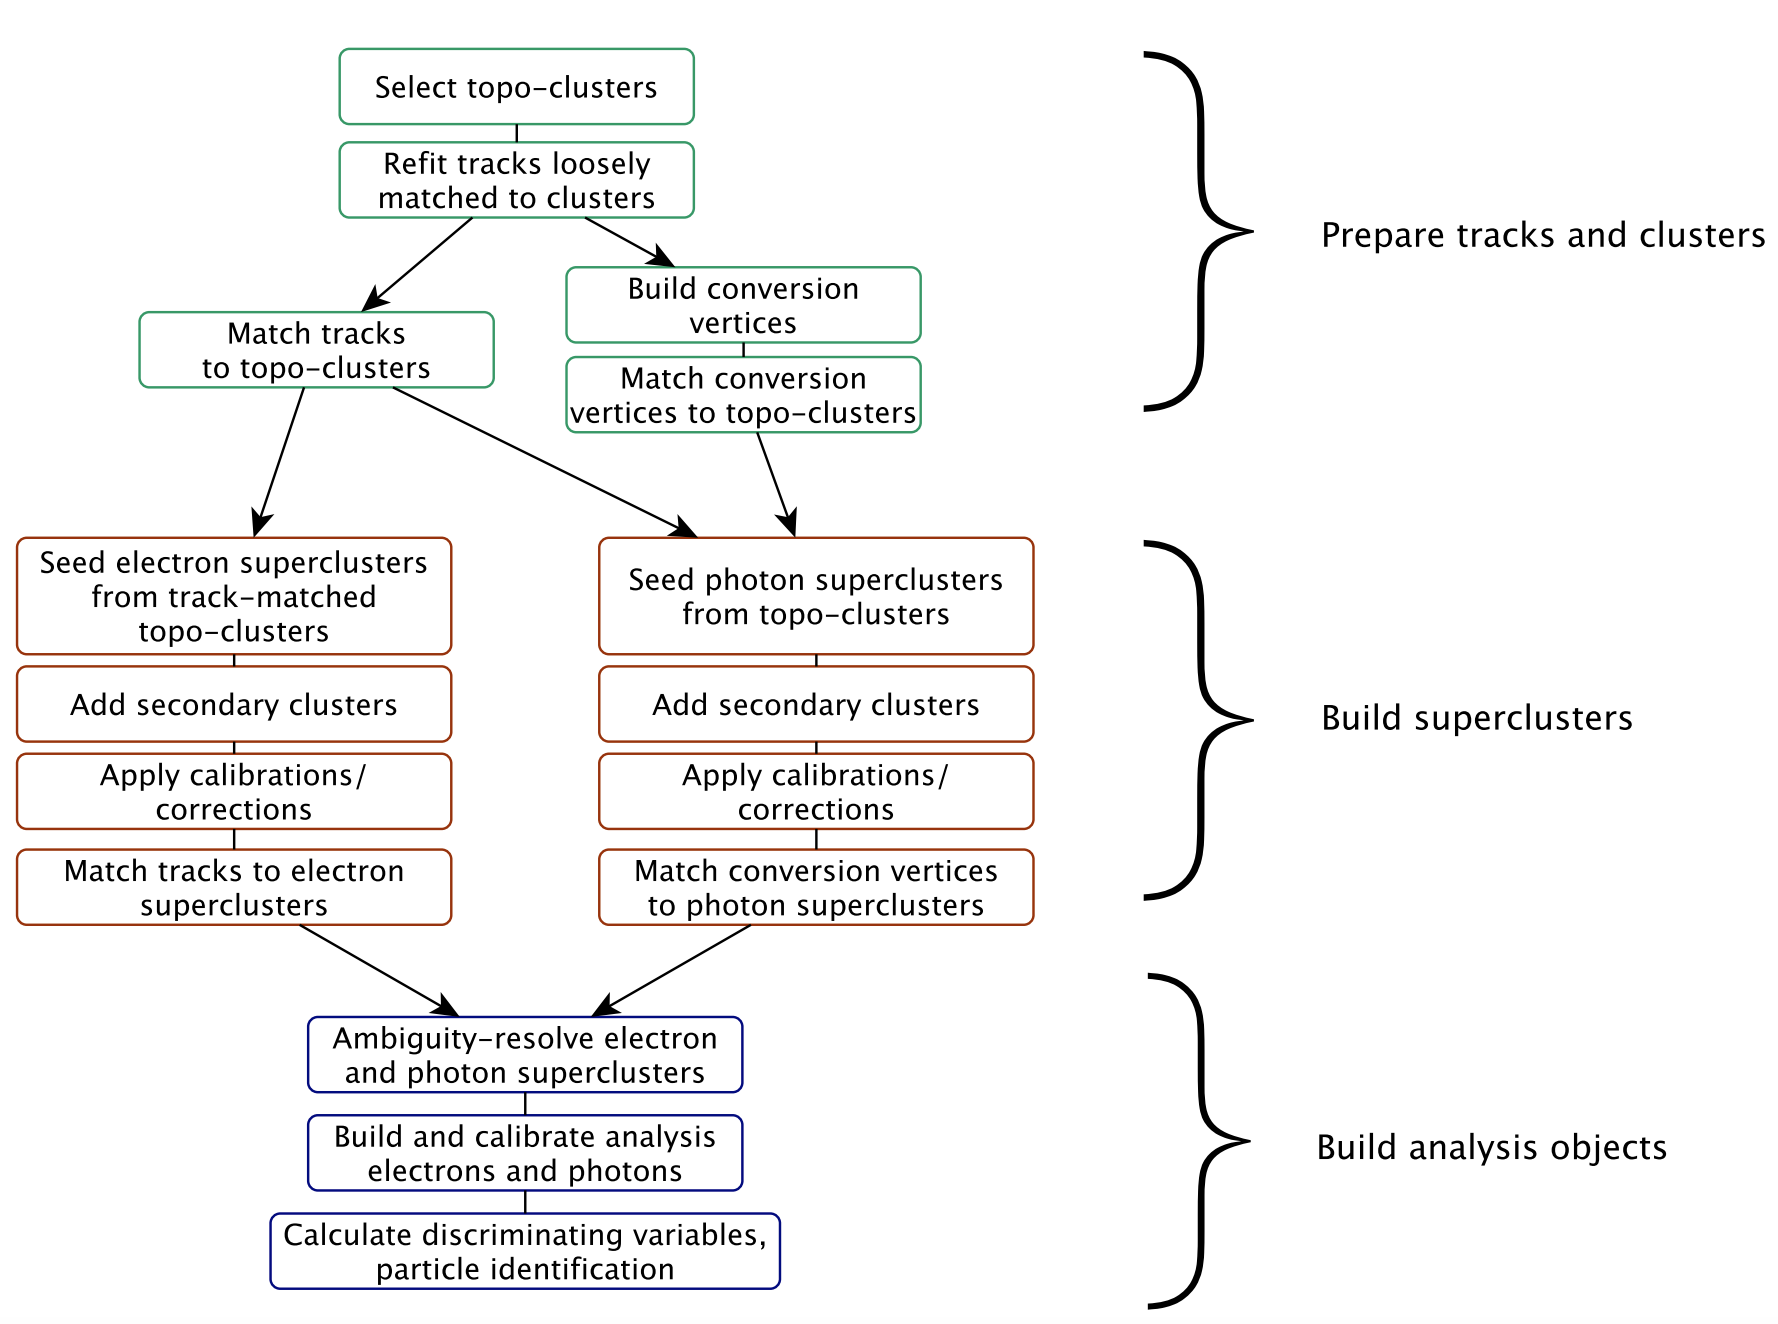
\includegraphics[width=0.8\textwidth,keepaspectratio]{topoclusters.png}
 	 	\caption[Topocluster reconstruction]{The algorithm scheme for topocluster reconstruction.}
 	 	\label{fig::topocluster}
 	 \end{figure}
 	 The algorithm for topocluster reconstruction \cite{topoclust2_2016}, \cite{topoclust_2019} starts with composing proto-clusters in the calorimeter using the noise threshold:
 	 \begin{equation}
 	 	\zeta_{cell}^{EM} =\frac{E_{cell}^{EM}}{\sigma_{noise,cell}^{EM}},\\
 	 \end{equation}
 	 where $E_{cell}^{EM}$ is the cell energy at the EM scale and $\sigma_{noise,cell}^{EM}$ is the expected cell noise. The latter comprises the electronic and the pile-up noise estimate based on the expected instantaneous luminosity. The proto-cluster is formed around a cell with $|\zeta_{cell}^{EM} \ge 4|$. Then the neighbouring cells are added to the proto-cluster. If an added cell passes the requirement of $|\zeta_{cell}^{EM} \ge 2 |$ then it serves as a seed for the next iteration, collecting all of its neighbours to the proto-cluster. If the two proto-clusters share a cell with $|\zeta_{cell}^{EM} \ge 2|$ then these proto-clusters are merged together. Proto-clusters with two local maxima are split into two clusters. For a proto-cluster to be considered as the EM topocluster it must have at least 50\% of its energy being contained in the \gls{emc}.
 	At the stage of track reconstruction the tracks are first extended and fitted with the global $\chi^2$ fitter using the pion hypothesis \cite{Cornelissen:2008zza}. If it fails, then a more complicated pattern reconstruction algorithm based on Kalman filter is used \cite{Cornelissen:1020106}. This algorithm uses the electron hypothesis and allows up to 30\% energy loss at each material surface. Then the tracks are loosely matched to the EM clusters if they meet one of the following criteria:
 	\begin{itemize}
 		\item The tracks extrapolated to the second layer of the \gls{emc} are consistent in $\phi$ and $\eta$ (matching in $\eta$ is not required for TRT-only tracks). 
 		\item The extrapolated tracks are consistent in $\phi$ (with a bit tighter requirements) and $\eta$ after rescaling the track momentum to cluster momentum.
 	\end{itemize}
  	Matching in $\phi$ coordinate assumes charge asymmetry to account for different direction of possible Bremsstrahlung radiation for positive and negative particles. Then the loosely matched tracks that have at least four silicon hits are refitted using the optimized \gls{gsf} \cite{GSF}, that allows to better take into account the energy losses in solid material.
  	
 	\subsubsection{Track-cluster matching}
 	Once the track is fitted with the \gls{gsf} algorithm the final matching with the cluster is performed using tighter matching requirements between the track and the cluster barycentre. If matching criteria are met with two or more tracks then the ambiguity resolving algorithm is used. This algorithm takes into account a number of parameters like the distance between the cluster barycentre and the track in $\phi$ and $\eta$, number of hits in the silicon detector and in the innermost silicon layer, association to photon conversion vertex, $E/p$ ratio and $p_T$. This allows to exclude converted photons as electron candidates and also helps to maintain high photon reconstruction efficiency. After track-cluster matching the electron cluster is extended around the seed to $3 \times 7$ in the barrel region or $5\times 5$ in the end-cap region by adding one row of the cells on each side. 
 	
 	\subsubsection{Supercluster reconstruction}
 	\begin{figure}[htbp]
 		\centering
 		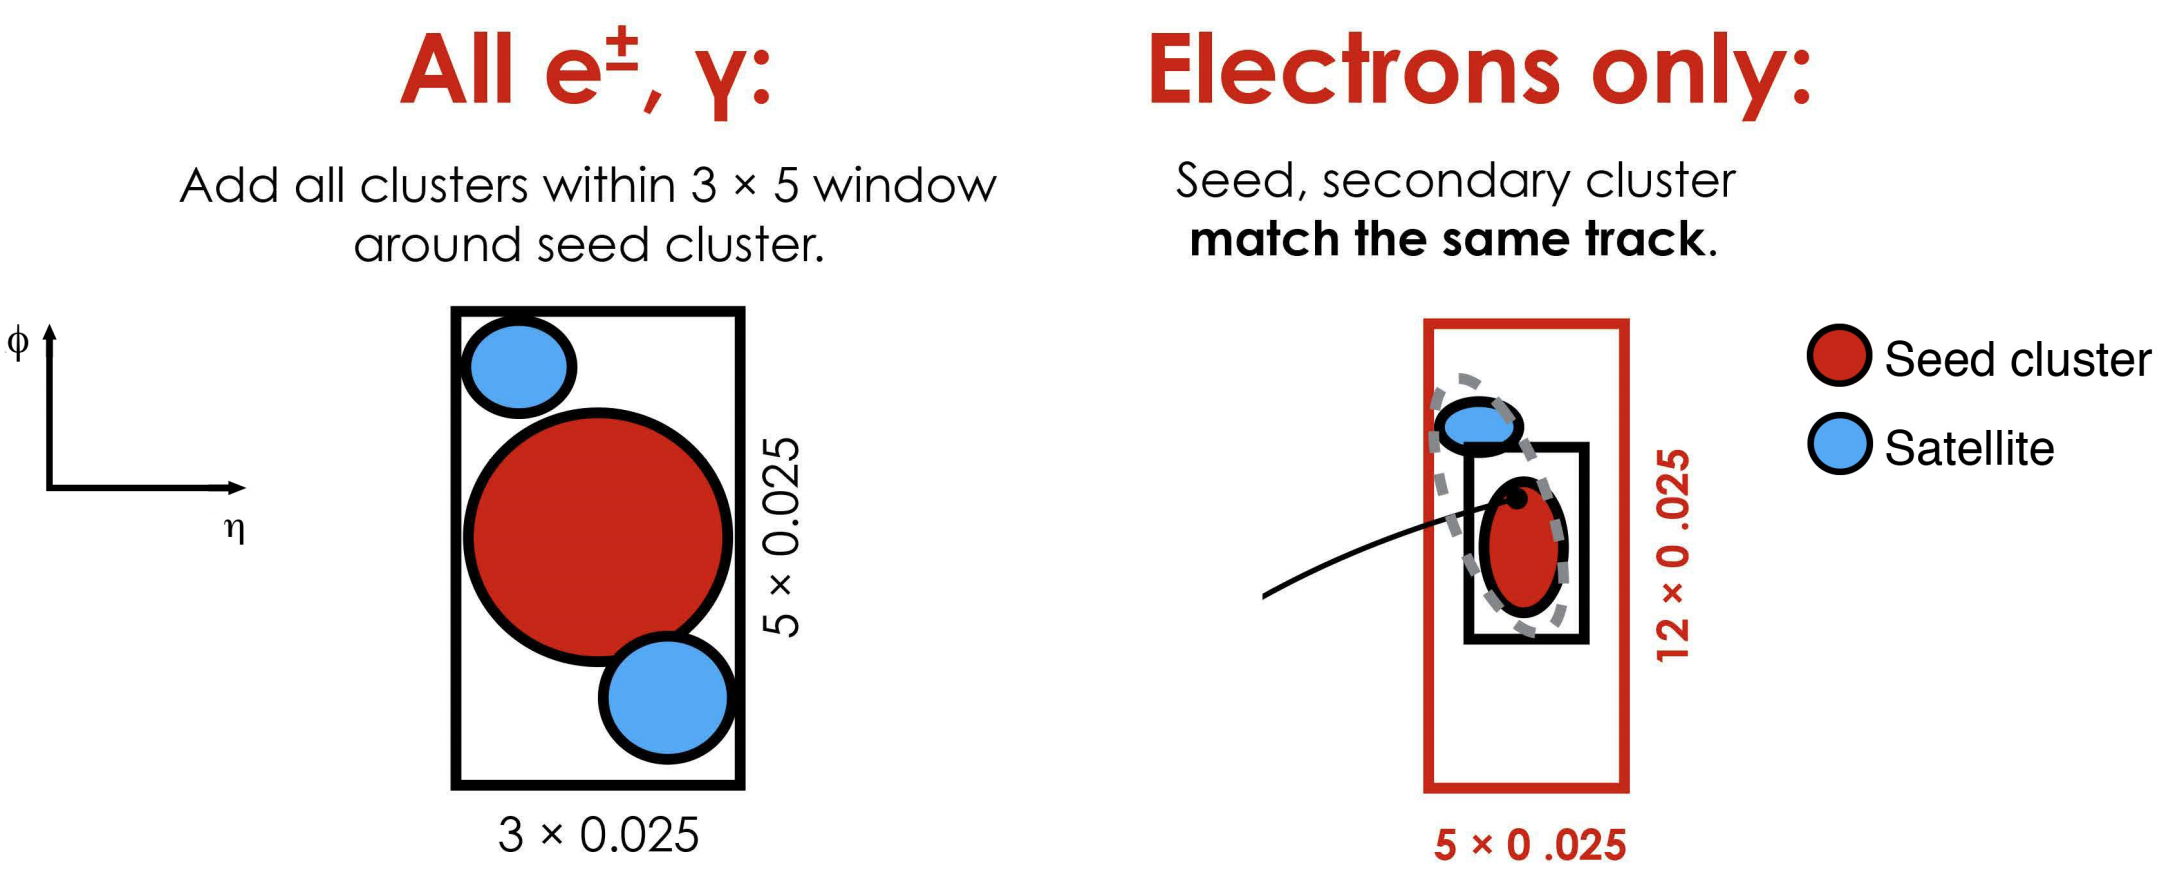
\includegraphics[width=\textwidth,keepaspectratio]{supercluster_el.png}
 		\caption[Supercluster reconstruction]{Supercluster reconstruction for electrons. Seed clusters are shown in red, satellite clusters in blue.}
 		\label{fig::supercluster}
 	\end{figure}
 	The composition of an electron supercluster is performed in two stages: first, the candidate EM topocluster is tested to be used as a seed for the supercluster. In the second stage the nearby EM topoclusters can be identified as satellite clusters, emerging from Bremsstrahlung radiation or topocluster splitting.
 	
 	First the EM topoclusters are sorted by their $E_T$ in descending order. For the cluster to be considered a seed it must have $E_T>1$ GeV, must be matched to a track with at least four hits in the silicon detectors and should not be assigned as a satellite cluster to any other seed. If these requirements are met then the algorithm described in Fig. \ref{fig::supercluster} is started. First, all topoclusters within a window of  $\Delta \eta \times \Delta \phi = 0.075 \times 0.125$ around the seed cluster barycentre are added as satellite cluster, as they most probably represent secondary EM showers coming from the same initial electron. Also, if a cluster within $\Delta \eta \times \Delta \phi = 0.125 \times 0.3$ window around the seed cluster barycentre share the "best-matched" track with the seed cluster - it is also added as a satellite.
  	Finally the energy of the reconstructed cluster must be calibrated. The calibration is performed using a multivariate technique based on data and MC samples using $Z \rightarrow ee$ events \cite{Aaboud:2018ugz}, \cite {Aaboud:2018yqu}. The shower shapes and other discriminating variables are computed at this stage.
    \subsection{Electron identification}
    Prompt electrons in the central region of the ATLAS detector ($|\eta|<2.47$) are selected using a likelihood-based (LH) identification. The LH uses a number of inputs from \gls{id} and calorimeter detectors, as well as combined information from both detectors (see Table 1 in \cite{electrons_reco1}). The \gls{pdfs} for the likelihoods of Run 2 were obtained using the simulated events.
    
    The electron LH is based on the products of n \gls{pdfs} P for signal $L_S$ and background $L_B$:
    \begin{equation}
    L_{S(B)}(\textbf{x}) = \prod_{i=1}^n P^i_{S(B)}(x_i),\\
    \end{equation}
    where $\textbf{x}$ is the vector of the LH input parameters, $P^i_{S}$ and $P^i_{B}$ are the pdf values for parameter $i$ at value $x_i$ for signal and background respectively.
    The LH operates at a number of working points, the higher the likelihood - the lower is the efficiency. For example, the efficiencies for identifying a prompt electron with $E_T=40$ GeV for Loose, Medium and Tight working points are 93\%, 88\% and 80\% respectively. Prompt electrons are assumed to come from the signal, while background includes the jets that mimic the prompt electrons, electrons from photon conversions and non-prompt electrons from hadron decays. For each electron candidate a discriminant $d_L$ is composed:
     \begin{equation}
    d_L=\frac{L_S}{L_S+L_B},\\
    \end{equation}
    that defines the electron likelihood identification. This discriminant $d_L$ has a sharp peak at unity for the signal and at zero for the background, which is not very convenient for picking working points. That is why the discriminant distribution is transformed using the inverse sigmoid function:
     \begin{equation}
    d_L^{\prime}=-\tau^{-1}\ln{(d^{-1}_L-1)},\\
    \end{equation}
    where $\tau=15$. Each operating point is assigned with a $d'_L$ value - if a discriminant exceeds this value for a given electron then this electron is considered signal.
    
    There are two advantages of using likelihood-based approach comparing to selection-criteria-based ("cut-based") identification:
    \begin{itemize}
    	\item The drawback of a cut-based approach is that if an electron fails to pass one of the cuts - it is definitely removed from the selection, while in the LH approach it is still possible for this electron to pass the selection thanks to other parameters. This quality promotes the selection efficiency. 
    	\item In case of a significant overlap in signal and background distribution of a certain parameter using it in a cut-based identification would entail large losses in efficiency. In the likelihood-based identification this parameter may be added without penalty. 
	\end{itemize}
	The likelihood input parameters were obtained from the simulated events, which means that real distributions in data may differ due to various mismodelling effects. These effects must be corrected in order to get an accurate and efficient identification. Mismodelling may depend on coordinates or energy. Chapter 5 of this dissertation is dedicated to the correction of electromagnetic shower shapes in the calorimeter, which are among the likelihood input parameters.
    \subsection{Electron isolation}
    Electron isolation plays a very important role in background suppression in physics analyses. Since electrons are reconstructed using the information from two different detectors - two different isolation definitions are possible, track-based and calorimeter-based. Let's first consider calorimeter-based isolation.
    
	 \begin{figure}[htbp]
		\centering
		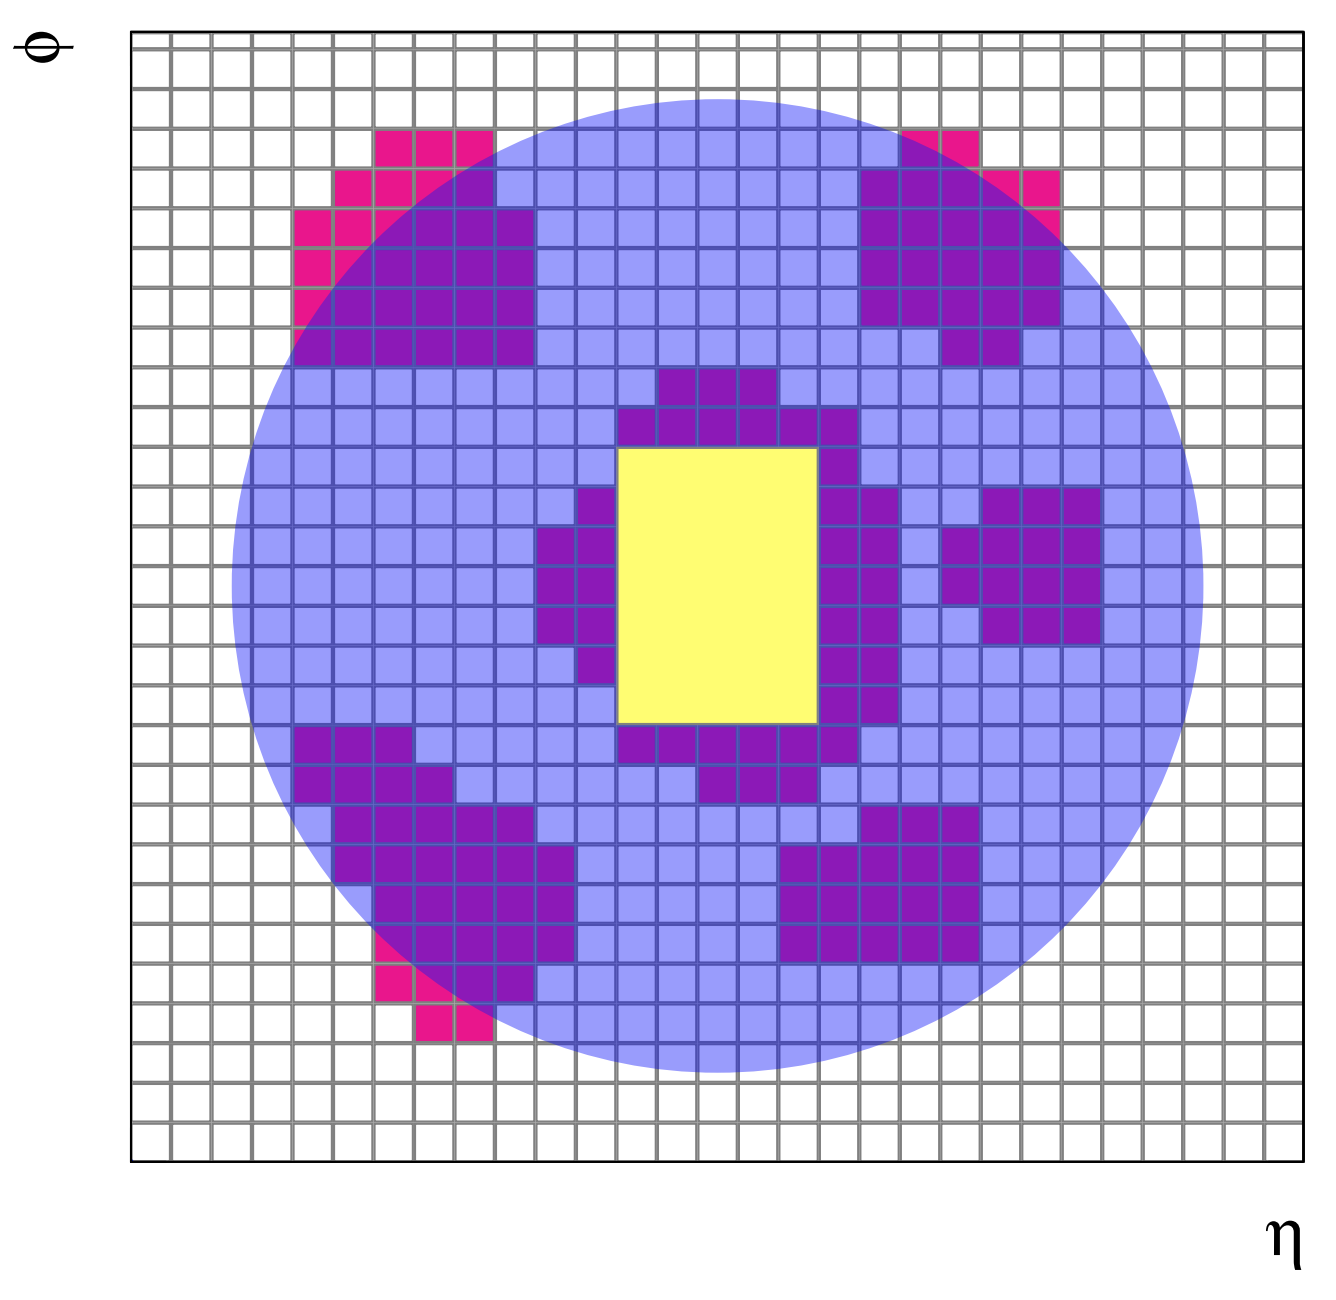
\includegraphics[width=0.5\textwidth,keepaspectratio]{calo_iso.png}
		\caption[Isolation cone]{The isolation cone is centred at the candidate electron. All topological clusters, shown in red, are included in the raw isolation variable. The $5\times 7$ cells included into core subtraction method are marked in yellow~\cite{topoclust_2019}.}
		\label{fig::calo_iso}
	\end{figure}
	As depicted in Fig. \ref{fig::calo_iso} the raw isolation energy $E_{isol}^{T,raw}$ includes the energy of all the topoclusters, barycentres of which fall within the isolation radius $\Delta R$. It also includes core energy of the electron candidate $E_{isol}^{T,core}$ which comprises the $5\times 7$ cells within the area of $\Delta \eta \times \Delta \phi = 0.125 \times 0.175$. The fixed size of the core ensures simplicity and stability, although it may happen that the topocluster is larger than the size of the core resulting in attributing the proper energy of the electron to the outside activity. This leakage effect is corrected for using no pile-up simulated events, parametrizing the leakage with a Crystal Ball function as a function of the transverse energy $E_{T,leakage}=E_{T,leakage}(E_T)$.
	
	Another effect that must be corrected for is the pile-up and underlying event contribution. This contribution is estimated from from the ambient energy density \cite{Cacciari:2007fd}. In every event all positive-energy topological clusters are taken into account in the entire range of calorimeter acceptance  $|\eta|<5$ using the $k_t$ jet clustering algorithm with a radius parameter $R=0.5$ and no jet $p_T$ threshold. Then for every jet its area $A$ is estimated and the jet energy density $\rho=p_T/A$ is computed. Using the information on the jet energy density together with the location of every jet one can obtain the median energy density $\rho_{median}(\eta)$ - a rapidity-dependent estimate of jet densities for every event. Then the pile-up correction can be evaluated in the following way:
	\begin{equation}
		E_{T,pile-up}(\eta)=\rho_{median}(\eta)\times(\pi \Delta R^2 - A_{core}),
	\end{equation}
	where $\Delta R$ is the radius of the isolation cone, and $A_{core}$ is the area of the subtracted signal core. Finally the calorimeter isolation variable may be defined as follows:
	\begin{equation}
		E^{isol}_{T,cone}=E^{isol}_{T,raw}-E_{T,core}-E_{T,leakage}-E_{T,pile-up}.
	\end{equation}
	The track-based isolation includes all tracks with $p_T>1$ GeV, within the fiducial region of the \gls{id}, that satisfy basic track quality requirements. Pile-up is mitigated by requiring that $|z_0\sin{\theta}|<3$ mm, to ensure that the track originates from the primary vertex. The track-based isolation is composed of all the tracks that fall within the radius $\Delta R$ excluding the candidate electron track.
	
	The own contribution of the candidate track into the isolation must also include possible Bremsstrahlung radiation emitted by the candidate electron. For that reason the tracks are extrapolated to the second layer of the \gls{emc} and if they fall within a window of $\Delta \eta \times \Delta \phi = 0.05 \times 0.1$ around the cluster position. The resulting variable is called $p_T^{isol}$.
	
	The track-based isolation allows to use variable-size cone, making the cone smaller for boosted particles. The cone size for the $p_{T,var}^{isol}$ would be:
	\begin{equation}
		\Delta R=min\left(\frac{10 GeV}{p_T[GeV]},R_{max}\right),
	\end{equation}
	where $R_{max}$ is the maximum cone size and may vary depending on the analysis needs, typically between 0.2 and 0.4.
      \section{Particle flow objects}
      \label{sec:pfo}
      The measurement of hadronic objects and particle showers remains a complicated task due to the large variety of particle types and properties they posses and because of the large energy/momentum span of the measured objects. For the low-energy charged particles the \gls{id} shows better momentum resolution and angular resolution. On the other hand, the calorimeter shows better performance at high energy and is also capable of detecting neutral particles. The idea behind the \gls{pf} algorithm \cite{pflow} is to combine the information from the two detectors to obtain the best result possible. To properly take into account every particle it has to be ensured that every particle detected in both detectors is counted only once. This means that for a charged particle its deposit in the calorimeter must be found and subtracted. The \gls{pfo} reconstruction process is schematically presented in Fig. \ref{fig::pflow}.
      	\begin{figure}[htbp]
      	\centering
      	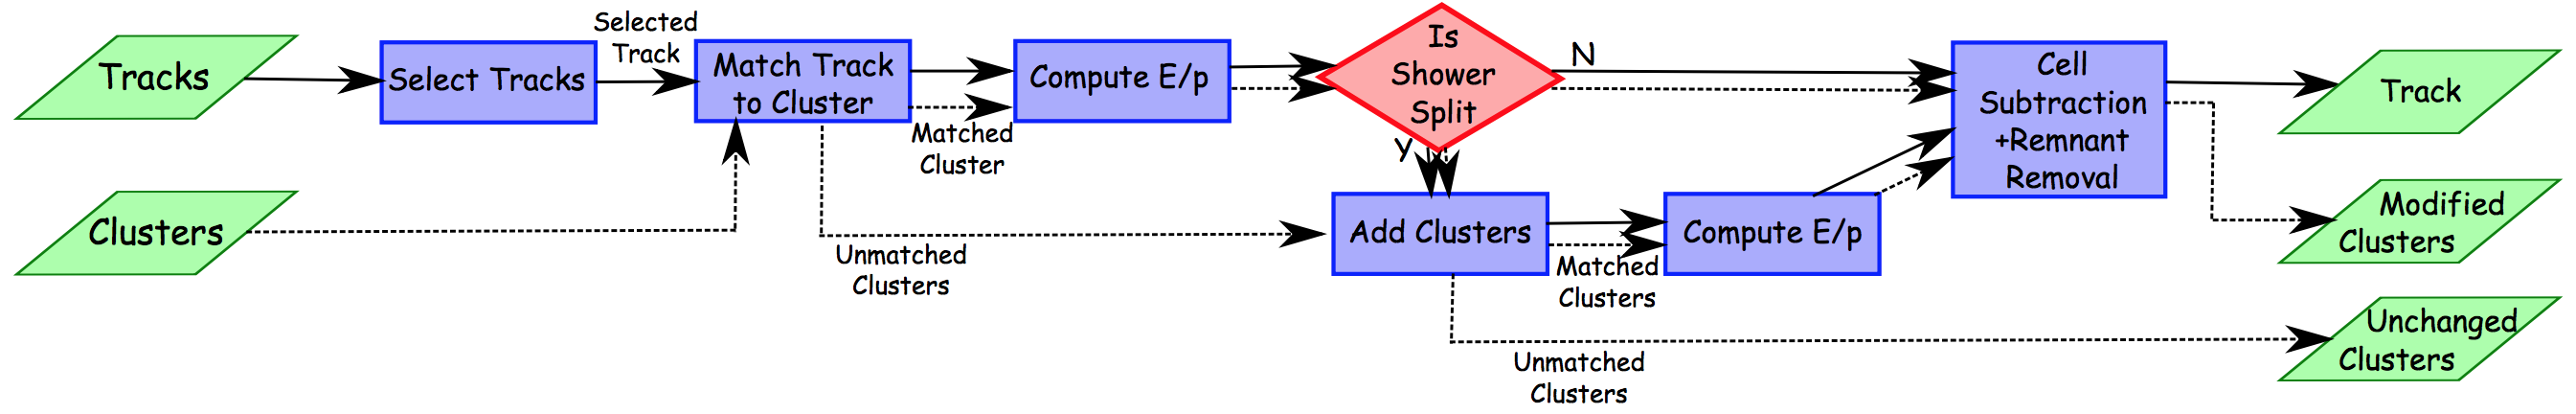
\includegraphics[width=1\textwidth,keepaspectratio]{pflow.png}
      	\caption[Particle flow algorithm]{The algorithm scheme for particle flow object reconstruction~\cite{pflow}.}
      	\label{fig::pflow}
      \end{figure}
  	  The process starts with getting \textit{tight} tracks from the \gls{id}, meaning these tracks must have at least nine hits in the silicon detectors and no holes n the pixel detector. The tracks must have $|\eta| < 2.5$ and $0.5 < p_T < 40$ GeV, corresponding to the kinematic region where tracks offer better resolution than the calorimeter. The tracks associated to leptons are removed. 
  	  
  	  The calorimeter topoclusters reconstructed like it was described in section \ref{sec::topocluster} and calibrated using the EM scale are matched to the tracks based on their spacial position and measured momentum. First the ranked based on a distance metric:
  	  	\begin{equation}
  	  \Delta R'=\sqrt{\left(\frac{\Delta \phi}{\sigma_{\phi}}\right)^2+\left(\frac{\Delta \eta}{\sigma_{\eta}}\right)^2},
  	  \end{equation}
  	  where $\Delta \phi$ and $\Delta \eta$ are the angular distances between the topocluster barycentres and the track, $\sigma_{\phi}$ and $\sigma_{\eta}$ are uncertainties in topocluster width. Preliminary matching is reached by requiring that $E^{clus}/p^{trk}>0.1$, where $E^{clus}$ is the cluster energy and $p^{trk}$ is the track momentum.\\
  	  It often happens, that energy deposit of a particle is split between two (most often) or more clusters. Then a split shower recovery procedure is initiated, looking for matching clusters in the radius of $\Delta R = 0.2$ around the track extrapolated to the second layer of the \gls{emc}. Then it is estimated if the energy of the track and the energy of the associated topocluster is consistent. If it is the case then the topoclusters matched to the tracks are removed. 
  	  
  	  Eventually two particle collections are obtained: a collection of charged particle flow objects (cPFOs) each with an associated track and neutral particle flow objects (nPFOs) with a calorimeter deposit. The former must also match the primary vertex, having $|z_0\times \sin{\theta}| < 2$ mm. The full procedure is described in detail in~\cite{pflow}.